\documentclass{article}
\usepackage[utf8]{inputenc}
\usepackage{multicol}
\usepackage{listings}
\usepackage{amssymb}
\usepackage{enumitem}
\usepackage{graphicx}
\usepackage{amsthm}
\usepackage{hyperref}

\usepackage{tikz}
\usetikzlibrary{arrows}

\usepackage[ruled,vlined]{algorithm2e}
\newtheorem{theorem}{Theorem}
\newtheorem{definition}{Definition}



%=====================================
%
%             Assignment 2
%
%     Author: Alexis Linard
%             a.linard@cs.ru.nl
%
%=====================================

\begin{document}

\title{Weekly Assignment 2}
\author{Tony Lopar s1013792}
\date{14th September 2017}
\maketitle

\paragraph{Deadline:} 20th September 2017, 6pm.

\section*{Exercise 1.}
Let us consider the following algorithm, creating a list of $n$ elements :

\begin{algorithm}
 \SetKwInOut{Input}{input}
 \SetKwInOut{Output}{output}
 \SetKwInOut{Parameter}{type}
 \SetKwFunction{New}{New}

 \Parameter{simple\_list\vspace*{-0.2cm}
 \begin{itemize}
	 \item self.next: \textbf{simple\_list}\vspace*{-0.4cm}
     \item self.key: \textbf{integer}
 \end{itemize}
 }

 element $\leftarrow$ \New(simple\_list) \;
 element.next $\leftarrow$ null \;
 element.key $\leftarrow$ 0 \;
 first $\leftarrow$ element \;
 temp $\leftarrow$ element \;

 \For{$i\leftarrow 1$ \KwTo $n-1$}{

	element $\leftarrow$ \New(simple\_list) \;
	element.next $\leftarrow$ null \;
	element.key $\leftarrow$ $i \times i$ \;
	temp.next $\leftarrow$ element \;
	temp $\leftarrow$ element \;

 }

 \caption{Playing with lists.}
\end{algorithm}
\vspace{-0.5cm}


\begin{enumerate}
\item What is the complexity of this algorithm?
\item Write an algorithm running over the list and displaying\footnote{you can use function \texttt{WriteLn(variable)} writing the content of \texttt{variable} in the terminal.} the key of each element.
\item Write an algorithm adding ``$1000$'' at the \textbf{beginning} of the list (hence list has $n+1$ elements). What is the complexity of the algorithm?
\item Write an algorithm adding ``$1000$'' to the \textbf{end} of the list (hence list has $n+1$ elements). What is the complexity of the algorithm?
\item Propose an improvement of the algorithm to reduce the complexity of adding an element to the end of the list to $\mathcal{O}(1)$.
\end{enumerate}

\subsection*{Solutions exercise 1}
\begin{enumerate}
    \item The complexity of this algorithm is $O(n)$, because the number of executions for the for-loop is depending on the input
    \item
    \begin{algorithm}
     \SetKwInOut{Input}{input}
     \SetKwInOut{Output}{output}
     \SetKwInOut{Parameter}{type}
     \SetKwFunction{New}{New}

     \Parameter{simple\_list\vspace*{-0.2cm}
     \begin{itemize}
    	 \item self.next: \textbf{simple\_list}\vspace*{-0.2cm}
         \item self.key: \textbf{integer}
     \end{itemize}
     }

     current $\leftarrow$ self.key \;

     \While{current.next $\neq$ null}{
        $WriteLn(element.key)$ \;
        current $\leftarrow$ current.next \;
     }

     \caption{Display all keys.}
\end{algorithm}
\vspace{-0.5cm}
    \item
    \begin{algorithm}
     \SetKwInOut{Input}{input}
     \SetKwInOut{Output}{output}
     \SetKwInOut{Parameter}{type}
     \SetKwFunction{New}{New}

     \Parameter{simple\_list\vspace*{-0.2cm}
     \begin{itemize}
    	 \item self.next: \textbf{simple\_list}\vspace*{-0.2cm}
         \item self.key: \textbf{integer}
     \end{itemize}
     }

    first $\leftarrow$ self.key \;
    element $\leftarrow$ \New(simple\_list) \;
    element.key $\leftarrow$ key \;
    element.next $\leftarrow$ first \;
    first $\leftarrow$ element \;


     \caption{Add element on first position.}
\end{algorithm}
\vspace{-0.5cm}
    The complexity of this algorithm is $O(1)$, because we already have a reference to the first element of the list. This means we can add an element and assign the old first element as next to it.
    \item
    \begin{algorithm}
     \SetKwInOut{Input}{input}
     \SetKwInOut{Output}{output}
     \SetKwInOut{Parameter}{type}
     \SetKwFunction{New}{New}

     \Parameter{simple\_list\vspace*{-0.2cm}
     \begin{itemize}
    	 \item self.next: \textbf{simple\_list}\vspace*{-0.2cm}
         \item self.key: \textbf{integer}
     \end{itemize}
     }

    first $\leftarrow$ self.key \;
    element $\leftarrow$ \New(simple\_list) \;
    element.key $\leftarrow$ key \;
    element.next $\leftarrow$ first \;
    current $\leftarrow$ element \;
    \While{$current.next \neq null$}{
        current $\leftarrow$ current.next
    }
    current.next $\leftarrow$ $\New(element)$


     \caption{Add element on last position.}
\end{algorithm}
\vspace{-0.5cm}
    The complexity of this algorithm is $O(n)$, because we need to traverse to the last element and add our new element as next of this old last value.
    \item An improvement could be to create a pointer to the last element. By creating this pointer we don't need to traverse to the last element, so we can access this element immediately and add a new element as next value.
\end{enumerate}

\section*{Exercise 2.}
Let us consider the following (incomplete) program:
\vspace{0.5cm}



\begin{algorithm}[htp]
  \DontPrintSemicolon
  \SetKwInOut{Parameter}{variable}
  \SetKwFunction{algo}{algo}
  \SetKwFunction{proc}{proc}
  \SetKwFunction{createStack}{createStack}
  \SetKwFunction{isEmpty}{isEmpty}
  \SetKwFunction{push}{push}
  \SetKwFunction{pop}{pop}
  \SetKwFunction{top}{top}
  \SetKwFunction{display}{display}
  \SetKwFunction{WriteLn}{WriteLn}
  \SetKwFunction{clear}{empty}
  \SetKwFunction{SetLength}{SetLength}

  \Parameter{stack: \textbf{array of strings} }
  \Parameter{no\_elements: \textbf{integer} }

 \tcc{creates empty stack}
  \SetKwProg{myproc}{Procedure}{}{}
  \myproc{\createStack{}}{
    no\_elements $\leftarrow$ 0 \;
    \SetLength{stack, no\_elements}  \tcp*{sets size of the array of strings "stack" to "no\_elements"}
  }

   \tcc{tests if the stack is empty (may return true of false)}
    \SetKwProg{myproc}{Function}{}{}
  \myproc{\isEmpty{}}{
    \If{no\_elements $>$ 0}{
        \KwRet{false}
        }\Else {
        \KwRet{true}
        }
  }

  \tcc{pushes "element" to the stack}
   \SetKwProg{myproc}{Procedure}{}{}
  \myproc{\push{element}}{
  no\_elements $\leftarrow$ no\_elements + 1 \;
  \SetLength{stack, no\_elements} \;
    stack[no\_elements] = $element$ \;

  }

 \tcc{removes and returns last element on stack}
    \SetKwProg{myproc}{Function}{}{}
  \myproc{\pop{}}{
    temp $\leftarrow$ stack[no\_elements] \;
    stack[no\_elements] $\leftarrow null$ \;
    no\_elements $\leftarrow$ no\_elements - 1 \;
    \SetLength{stack, no\_elements} \;
    \KwRet{temp}
  }

  \tcc{returns top element}
   \SetKwProg{myproc}{Function}{}{}
  \myproc{\top{}}{
    \KwRet{stack[no\_elements]} \;
  }

  \tcc{displays elements in the stack}
   \SetKwProg{myproc}{Procedure}{}{}
  \myproc{\display{}}{
    \For{i $\leftarrow 1$ \KwTo $i \leftarrow no\_elements$}{
    \WriteLn{stack[i]}}
  }

  \tcc{Removes all values of the stack}
   \SetKwProg{myproc}{Procedure}{}{}
  \myproc{\clear{}}{
    \While{$no\_elements > 0$}{
        stack[no\_elements] $\leftarrow null$ \;
        $no\_elements \leftarrow no\_elements - 1$ \;
    }
  }


\createStack{}\;
\push{``AAA''}\;
\display{}  \tcp*{1}
\push{``BBB''}\;
\push{``CCC''}\;
\display{} \tcp*{2}
name $\leftarrow$ \pop{}\;
\WriteLn{name}\;
\display{} \tcp*{3}
  \caption{Stack as array of strings.}
\end{algorithm}
\vspace{-0.5cm}


\begin{enumerate}
\item Complete the functions and procedures above.
\item Give the complexity of each function.
\item What is displayed on the screen?\footnote{recall that \texttt{WriteLn(variable)} writes the content of \texttt{variable} in the terminal.}
\item Write a function $empty()$, emptying the stack.
\end{enumerate}

\subsection*{Solutions exercise 2:}
\begin{enumerate}
    \item See algorithm 5 for solution
    \item
        \begin{enumerate}[label=(\alph*)]
            \item Note: The complexity for each of the functions will be displayed as functionname: complexity. For the predefined function setLength the complexity will be assumed to be $O(n)$, since a bigger array needs to be created and all values copied to it and the function is not defined in the algorithm.
            \item createStack(): $O(n)$, since the function setLength is called and for this function the assumed complexity is $O(n)$
            \item isEmpty(): $O(1)$, because it only reads a value and returns it. The execution does not depend of the number of elements.
            \item push(element): $O(n)$, since for setLength it is assumed that the complexity will be $O(n)$.
            \item pop():$O(n)$, since for setLength it is assumed that the complexity will be $O(n)$. But, if we don't set the length of the array the complexity will reduce to $O(1)$.
            \item top(): $O(1)$, because the function only reads a certain value.
            \item display(): $O(n)$, because we loop through all elements of the stack in order to write them in the console.
        \end{enumerate}
    \item The following will be displayed on the screen: \\
    AAA \\
    AAABBBCCC \\
    CCC \\
    AAABBB
    \item See algorithm 5 for solution
\end{enumerate}

\newpage

\section*{Exercise 3.}
Let us consider the following (incomplete) program:

\begin{algorithm}[htp]
  \DontPrintSemicolon
  \SetKwInOut{Parameter}{type}
  \SetKwFunction{algo}{algo}
  \SetKwFunction{proc}{proc}
  \SetKwFunction{createStack}{createStack}
  \SetKwFunction{isEmpty}{isEmpty}
  \SetKwFunction{push}{push}
  \SetKwFunction{pop}{pop}
  \SetKwFunction{top}{top}
  \SetKwFunction{clear}{empty}
  \SetKwFunction{display}{display}
  \SetKwFunction{WriteLn}{WriteLn}

 \Parameter{stack\vspace*{-0.2cm}
 \begin{itemize}
	 \item self.next: \textbf{stack}\vspace*{-0.4cm}
     \item self.name: \textbf{string}
 \end{itemize}
 }

 \tcc{creates empty stack}
  \SetKwProg{myproc}{Procedure}{}{}
  \myproc{\createStack{}}{
    stack $\leftarrow$ null \;
  }

   \tcc{tests if the stack is empty (may return true of false)}
    \SetKwProg{myproc}{Function}{}{}
  \myproc{\isEmpty{}}{
    \If{stack.top $==$ 0}{
        \KwRet{true}
    }\Else {
        \KwRet{false}
        }
  }

  \tcc{pushes an element on top of the stack}
   \SetKwProg{myproc}{Procedure}{}{}
  \myproc{\push{element}}{
    stack.top = stack.top + 1 \;
    stack[stack.top] = element
  }

 \tcc{removes and returns 1st element on stack}
    \SetKwProg{myproc}{Function}{}{}
  \myproc{\pop{}}{
    \If{\isEmpty{}}{
        error
    } \Else{
        stack.top = stack.top - 1 \;
        \KwRet{stack.top + 1}
    }
  }

  \tcc{returns top element}
   \SetKwProg{myproc}{Function}{}{}
  \myproc{\top{}}{
    \KwRet{stack[stack.top]} \;
  }

  \tcc{display elements in the stack}
   \SetKwProg{myproc}{Procedure}{}{}
  \myproc{\display{}}{
    \For{$i \leftarrow 1$ \KwTo $stack.top$}{
        \WriteLn{stack[i]}
    }
  }

  \tcc{empties the stack}
   \SetKwProg{myproc}{Procedure}{}{}
  \myproc{\clear{}}{
    stack $\leftarrow$ null \;
  }


\push{``AAA''}\;
\display{}  \tcp*{1}
\push{``BBB''}\;
\push{``CCC''}\;
\display{} \tcp*{2}
name $\leftarrow$ \pop{}\;
\WriteLn{name}\;
\display{} \tcp*{3}

  \caption{Stack. }
\end{algorithm}

\begin{enumerate}
\item Complete the functions and procedures above.
\item Give the complexity of each function.
\item What is displayed on the screen?
\item Write a function $empty()$, emptying the stack.
\end{enumerate}

\newpage

\subsection*{Solutions exercise 3:}
\begin{enumerate}
    \item See algorithm 6 for solution
    \item
        \begin{enumerate}[label=(\alph*)]
            \item createStack(): $O(1)$, because the only operation is setting the value of stack to null
            \item isEmpty():, $O(1)$, because it only checks the top and returns if it's zero.
            \item push(element): $O(1)$, because the pointer for the top is being moved to the right and an element is assigned to the position.
            \item pop(): $O(1)$, because it only decreases the top and returns the old value.
            \item top(): $O(1)$, because it just returns the value.
            \item display(): $O(n)$, because to print all the values there is looped through all elements of the stack.
        \end{enumerate}
    \item The following will be displayed: \\
        AAA \\
        AAABBBCCC \\
        CCC \\
        AAABBB
    \item See algorithm 6 for solution
\end{enumerate}

\section*{Exercise 4.}
Apply BFS to the graph below.

\subsection*{Solutions exercise 4:}

\begin{enumerate}
\item We start at Vertex 1. The queue is empty and the only grey vertex is 1, since this is our start.
\item We loop through all adjecencies of 1, these are 2, 3, 4 and 1. Since 1 is already grey, we won’t do anything with it. We will make 2, 3 and 4 grey. We will also add the values 2, 3, 4 to the queue. The queue now contains: 2, 3 and 4.
\item All adjacencies passed, we make 1 black and we take the first element from the queue: 2. The queue now contains: 3 and 4.
\item We loop through all adjecencies of 2, since the only adjecency is itself, we won’t do anything with it because it’s already grey
\item We make 2 black and we take the first element from the queue: 3. The queue now contains: 4.
\item We loop through all adjecencies of 3 and find the vertices 5 and 6, so we make them grey and add them to the queue. The queue now contains: 4, 5, 6.
\item We make 3 black and take the next element from the queue: 4. The queue now contains: 5, 6.
\item We loop though all adjacencies of 4, this is only 3. 3 is already grey, so we won’t do anything with it.
\item We make 4 black and we take the next element from the queue: 5. The queue now contains: 6.
\item We loop through all vertices and find: 3 and itself, because 3 is black and 5 is already grey we won’t do anything with them.
\item We make 5 black and we take the next element from the queue: 6. The queue is now empty.
\item We loop through all vertices and find 3, 5 and 6. \item All these values are already grey of black, so we won’t do anything with them.
\item The queue is empty, so the process ends.
\end{enumerate}

Below is shown a visual representation with the shortest distance from the start to each vertex. All vertices are coloured black, because we already finished them all. Moreover the breadth-first tree is visualized in green.
\vspace*{-0.4cm}
\begin{figure}[h!]
\centering
\includegraphics[width=5cm]{images/[Algo]Week 2 Exercise 4.png}
\end{figure}
\vspace*{-1cm}

\newpage
\section*{Exercise 5.}

Give an example of a directed graph $G = (V,E)$, a source vertex $s \in V$, and a set of tree edges $E_{\pi} \subseteq E$ such that for each vertex $v \in V$, the unique simple path
in the graph $(V, E_{\pi})$ from $s$ to $v$ is a shortest path in $G$, yet the set of edges $E_{\pi}$ cannot be produced by running BFS on $G$, no matter how the vertices are ordered
in each adjacency list.

\subsection*{Solutions exercise 5:}
In order to explain my solution i've made the following graph:

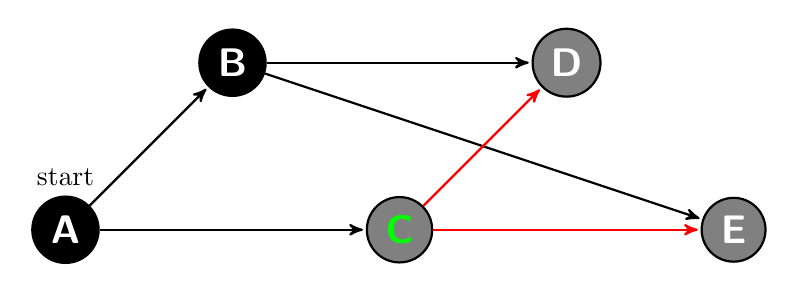
\begin{tikzpicture}[->,>=stealth',shorten >=1pt,auto,node distance=3cm,
                    thick,main node/.style={circle,draw,font=\sffamily\Large\bfseries}]

  \node[fill = black, text = white][main node] (2) {B};
  \node[fill = black, text = white][main node] (1) [below left of=2, label = start] {A};
  \node[fill = gray, text = green][main node] (3) [below right of=2] {C};
  \node[fill = gray, text = white][main node] (4) [above right of=3] {D};
  \node[fill = gray, text = white][main node] (5) [below right of=4] {E};

  \path[every node/.style={font=\sffamily\small}]
    (1) edge[black] node [left] {} (2)
        edge[black] node [above] {} (3)
    (2) edge[black] node {} (4)
        edge[black] node {} (5)
    (3) edge[red] node {} (4)
        edge[red] node {} (5);
\end{tikzpicture}
\newline
Given the source vertex A, the BFS starts with adding B or C to the queue. When processing B or C, vertices D and E are added to the queue. After this the remaining vertex (B or C) will be processed. This will lead to D and E, but both are already gray. The edges from the last vertex (B or C) to D and E won't be an element in the set $E_\pi$, because they are not included in the breath search tree.\\
\\*
The ignored edges could be: \\
(B,D), (B,E) when C is processed before B OR\\
(C,D), (C,E) when B is processed before C\\
\\*
So $E_\pi$ should contain at least one edge that can not be found from C before B and one from B before C.
$E_\pi = \{(A,B), (B,D), (A,C), (C,E)\} $

\newpage
\section*{Exercise 6.}
Give an algorithm returning, if it exists, the cycle of minimal length via a vertex $s$ given a graph $G$.\footnote{you can use the following functions: \begin{itemize} \item \texttt{New}($queue$) returning an empty queue. \item \texttt{enqueue}($Q$, $element$) adding $element$ to queue $Q$. \item \texttt{dequeue}($Q$) removing and returning and $element$ from $Q$.  \end{itemize}} Prove its correctness.

\subsection*{Solutions exercise 6:}

In this exercise we will create an algorithm that will return the minimum length of the cycle. First we need to all find possible cycles in the graph. We can detect possible cycles with the breadth-first-search algorithm. A cycle will be completed when two paths of BFS come across each other. This will be the case when we find an adjacent of the current vertex that is in a discovered state, because the last values of each path are marked as discovered.
\newline
In the graph below there will be a visual representation of this. The current vertex is B, this vertex has as a adjacent node D. Node D is already discovered by the path $A \rightarrow C \rightarrow D$, so this is the point where path $A \rightarrow C$ comes across the shortest path of D. Because we reached both vertices from A, node A will be also part of the cycle.
\newline
In the algorithm we have to check whether two paths will come across each other. If this is the case, we will return the list of predecessors for both paths, because both of these lists contain one half of the cycle. On the next page a pseudo-code implementation of this algorithm is shown in algorithm 7.
\newline
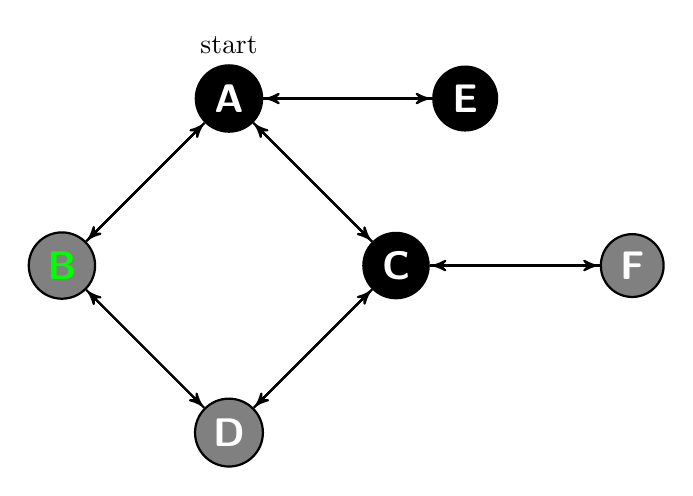
\begin{tikzpicture}[->,>=stealth',shorten >=1pt,auto,node distance=3cm, every loop/.style={},
                    thick, ,main node/.style={circle,draw,font=\sffamily\Large\bfseries}]

  \node[fill = black, text = white, label = start][main node] (1) {A};
  \node[fill = gray, text = green][main node] (2) [below left of=1] {B};
  \node[fill = black, text = white][main node] (3) [below right of=1] {C};
  \node[fill = gray, text = white][main node] (4) [below right of=2] {D};
  \node[fill = black, text = white][main node] (5) [ right of=1] {E};
  \node[fill = gray, text = white][main node] (6) [ right of=3] {F};

  \path[every node/.style={font=\sffamily\small}]
    (1) edge[black] node [left] {} (2)
        edge[black] node [above] {} (3)
        edge[black] node [above] {} (5)
    (2) edge[black] node {} (1)
        edge[black] node {} (4)
    (3) edge[black] node {} (1)
        edge[black] node {} (4)
        edge[black] node {} (6)
    (4) edge[black] node {} (2)
        edge[black] node {} (3)
    (5) edge[black] node {} (1)
    (6) edge[black] node {} (3);
\end{tikzpicture}

\begin{algorithm}[htp]
  \DontPrintSemicolon
  \SetKwInOut{Parameter}{type}
  \SetKwFunction{getPredecessors}{getPredecessors}
  \SetKwFunction{dequeue}{dequeue}
  \SetKwFunction{enqueue}{enqueue}
  \SetKwFunction{cycle}{cycle}
  \SetKwFunction{buildCycle}{buildCycle}

  \SetKwProg{myproc}{Function}{}{}
  \myproc{\cycle{G,s}}{
    \For{each vertex u in V[G]}{
      color[u] $\leftarrow$ white \;
    }

    color[s] $\leftarrow$ gray \;
    Q $\leftarrow$ \emptyset

    \enqueue(Q,s)

    \While{Q \neq $\emptyset$}{
      \textbf{let} u $\leftarrow$ \dequeue(Q) \;
      \For{each v $\in$ Adj[u]}{
      \If{color[v] = white}{
         color[v] $\leftarrow$ gray \;
         $\pi[v] \leftarrow$ u \;
         \enqueue(Q,v)
      }
      \ElseIf{color[v] = gray}{
         \KwRet{$\buildCycle(u,v)$}  \;
      }
      }
      color[u] $\leftarrow$ black \;
    }
  }

  \myproc{\buildCycle{}}{
    vertices $\leftarrow$ New (set) \;
    vertices.add($getPredecessors(u)$) \;
    vertices.add($getPredecessors(v)$) \;

    \KwRet{vertices} \;
  }

  \myproc{\getPredecessors{x}}{
    $vertices \leftarrow \New(set)$ \;
    vertices.add(x) \;

    temp = x \;
    \While{$\pi[temp]$ \neq nil}{
      temp = $\leftarrow \pi[temp]$ \;
      vertices $\leftarrow$ temp \;
    }
    \KwRet{vertices}
  }

  \caption{Find shortest cycle}
\end{algorithm}

\newpage

\section*{Exercise 7.}
Give an algorithm verifying if a undirected and connected graph has a cycle. Prove its correctness.

\subsection*{Solutions exercise 7:}
When we use the BFS algorithm on the graph, we can mark each element with a color, defining it's state. With BFS we can have multiple paths that search for the shortest path to each vertex. To check if we have a cycle we have to search where these paths can come across each other. The paths will come across each other when the vertex has an adjacent of the other path. Since the paths are coming closer to each other during the process, there must be a adjacent that's already grey when we meet the other path. Since the graph is undirected, we know that we can go through the cycle from both sides, so don't have to matter about directed edges. The situation is quite similar with the situation from exercise 6.
\newline
To create an algorithm for this process, we can take the algorithm of BFS and add a check for grey adjecents when we check all adjecents of a vertex. The function should return whether there is a cycle in the graph. If a grey adjecent is found for a vertex, then we will return true. When all vertices are finished and we haven't found a cycle, we will return false. The algorithm will be as follows:

\begin{algorithm}[htp]
  \DontPrintSemicolon
  \SetKwInOut{Parameter}{type}
  \SetKwFunction{getPredecessors}{getPredecessors}
  \SetKwFunction{dequeue}{dequeue}
  \SetKwFunction{enqueue}{enqueue}
  \SetKwFunction{cycle}{cycle}
  \SetKwFunction{buildCycle}{buildCycle}

  \SetKwProg{myproc}{Function}{}{}
  \myproc{\cycle{G,s}}{
    \For{each vertex u in V[G]}{
      color[u] $\leftarrow$ white \;
    }

    color[s] $\leftarrow$ gray \;
    Q $\leftarrow$ \emptyset

    \enqueue(Q,s)

    \While{Q \neq $\emptyset$}{
      \textbf{let} u $\leftarrow$ \dequeue(Q) \;
      \For{each v $\in$ Adj[u]}{
       \If{color[v] = white}{
         color[v] $\leftarrow$ gray \;
         $\pi$[v] $\leftarrow$ u \;
         \enqueue(Q,v)
       }
       \ElseIf{color[v] = gray}{
         \KwRet{true} \;
       }
      }
      color[u] $\leftarrow$ black
    }

    \KwRet{false} \;
  }
  \caption{Check whether there is a circle}
\end{algorithm}
\vspace{-0.5cm}

\end{document}
